\section{The IoT Vulnerability Reproduction Pipeline}
\label{sec:pipeline}

Reproducing an IoT vulnerability from nothing but a CVE identifier demands a chain of capabilities that existing security benchmarks never test. The agent cannot start from source code or a pre-built binary; it must locate proprietary firmware, unpack an undocumented container format, identify a foreign instruction set, and---critically---convince a cross-architecture binary to execute in an environment it was never designed for. \cref{fig:pipeline} maps the six stages an agent must traverse and the seven roadblocks where progress can halt.

\subsection{Stages and Roadblocks}

\cref{fig:pipeline} illustrates the complete reproduction pipeline.

\begin{figure}[t]
    \centering
    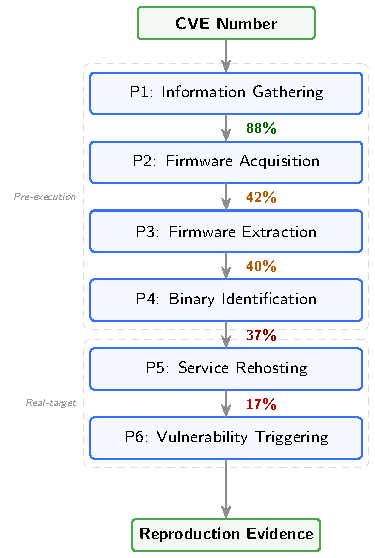
\includegraphics[width=\linewidth]{figures/pipeline.pdf}
    \caption{The IoT vulnerability reproduction pipeline. Agents receive a CVE number and must navigate six stages. Reach rates from 372 evaluated runs are shown on the arrows; the pipeline collapses at the rehosting stage (R5).}
    \label{fig:pipeline}
\end{figure}

\paragraph{Stage 1---Intelligence gathering.} The agent must map a CVE number to an affected device line, a firmware version, and a vulnerable endpoint. For CVE-2020-13389, this means learning that Tenda AC15 firmware v15.03.05.19 contains a stack overflow reachable through \texttt{/goform/openSchedWifi} in the embedded HTTP server. NVD entries provide a starting point, but agent trajectories show they also scrape vendor advisories, Exploit-DB posts, and Chinese-language security blogs---sources with varying completeness and accuracy. Roadblock \roadblock{1} (Version Identification) sits here: without the exact firmware version string, all downstream stages are misdirected.

\paragraph{Stage 2---Firmware acquisition.} The agent must locate and download the correct firmware image. Vendors remove old firmware from their sites, archive mirrors go stale, and some firmware sits behind login walls that agents cannot traverse. The 14.7~MB TRX blob for the Tenda AC15 lives on the vendor's download page---discoverable through search---but a D-Link SHRS-encrypted image from 2018 might have no remaining live download. Even locating the right file is non-trivial: vendor pages change structure between models, naming conventions are inconsistent, and agents sometimes download the correct model's firmware for the wrong hardware revision. Roadblock \roadblock{2} (Firmware Acquisition) captures this challenge.

\paragraph{Stage 3---Firmware extraction.} The raw blob must be unpacked. This is where firmware's heterogeneity bites hardest. Tenda ships TRX containers with LZMA-compressed SquashFS; D-Link uses SHRS encryption with a 128-byte XOR key embedded in the bootloader; Zyxel wraps JFFS2 in a custom header with a vendor magic number. \texttt{binwalk} handles the common cases but fails silently on encrypted payloads or vendor-proprietary formats. In our traces, agents that encounter an unrecognized magic byte often declare the file ``corrupt'' and abandon the run, when the actual problem is an unsupported compression mode or an offset they did not specify. Roadblock \roadblock{3} (Firmware Extraction) checks whether the agent correctly unpacks the container layers and decrypts encrypted payloads.

\paragraph{Stage 4---Architecture and binary identification.} Inside the extracted rootfs, the agent must determine the CPU architecture and pick out the vulnerable binary. The answer is rarely \texttt{x86\_64}. Our corpus spans MIPS32 (42\% of tasks), ARM (31\%), AArch64 (16\%), and x86 (11\%). The Tenda AC15 runs a MIPS32 little-endian toolchain; its \texttt{httpd} binary sits at \texttt{/usr/bin/httpd} and links against uClibc. Agents typically run \texttt{file} on a candidate binary---correctly identifying MIPS32-LE about 89\% of the time---but they rarely follow through by matching the binary's linked libraries against what exists in the extracted rootfs, which is the first step toward rehosting. Roadblock \roadblock{4} (Binary Identification) verifies both the architecture claim and that the agent located the correct vulnerable binary.

\paragraph{Stage 5---Service rehosting.} This is where the pipeline collapses. The agent must make the vulnerable service executable so it can receive a crafted input and trigger the bug. Three paths exist. \emph{Full-system emulation} (FirmAE/QEMU system mode) boots the entire firmware image with a substituted kernel---the approach that works for 79\% of firmware in the FirmAE evaluation~\cite{firmae}, provided the agent correctly configures the NVRAM partition, network bridge, and kernel module dependencies. \emph{User-space emulation} (QEMU user mode) runs only the target binary, but demands that every dynamically-linked library is resolved and that the emulator's endianness and CPU variant match exactly. \emph{Static analysis} is the fallback: read the disassembly, understand the bug, and reason about exploitability without execution---the path agents default to when both emulation modes fail.

Roadblock \roadblock{5} (Service Rehosting) subsumes the many distinct failure points of emulation: library resolution, NVRAM initialization, peripheral stubs, kernel module dependencies, and network stack configuration. Each has a mature tool---\firmwell handles multi-process dependency resolution, \textsc{Penguin} automates NVRAM configuration, \textsc{Pandawan} augments the kernel for module support, and \textsc{Pemu} provides network device emulation---yet our experiments show these tools are almost never used effectively by LLM agents.

\paragraph{Stage 6---Exploitation.} Once the service is rehosted and reachable, the agent must deliver a proof-of-concept that triggers the vulnerability (Roadblock \roadblock{6}), and optionally develop a full exploit achieving code execution or authentication bypass (Roadblock \roadblock{7}). Under validity gating (\cref{sec:rrs}), triggering and exploitation credit is only awarded when the PoC executes against the \emph{rehosted real firmware}. Agents that substitute a host-native simulation receive no exploitation credit---a design choice we return to in \cref{sec:experiments} when we show that 62\% of runs take exactly that shortcut.

\subsection{Roadblock Taxonomy}
\label{sec:roadblocks}

\cref{tab:roadblocks} catalogues the seven roadblocks. Difficulty is calibrated against what an expert with the corresponding tool can achieve: Format and Architecture Detection are Easy because \texttt{binwalk~-e} and \texttt{file} handle most firmware; Service Rehosting is Very Hard because it demands configuration-specific debugging across heterogeneous hardware abstractions, even with a mature tool like \firmae.

\begin{table}[t]
    \centering
    \caption{Roadblock taxonomy. Diff.: E (Easy), M (Medium), H (Hard), VH (Very~Hard). SOTA tools in \cref{sec:roadblocks}.}
    \label{tab:roadblocks}
    \footnotesize
    \begin{tabular}{cllc}
        \toprule
        \textbf{ID} & \textbf{Roadblock} & \textbf{Stage} & \textbf{Diff.} \\
        \midrule
        \roadblock{1} & Info.\ Gathering      & Intel.\     & M  \\
        \roadblock{2} & FW Acquisition        & Acquire     & M  \\
        \roadblock{3} & FW Extraction         & Extract     & H  \\
        \roadblock{4} & Binary ID             & Identify    & E  \\
        \roadblock{5} & Service Rehosting     & Rehost      & VH \\
        \roadblock{6} & Vuln.\ Triggering     & Exploit     & H  \\
        \roadblock{7} & Exploit Development   & Exploit     & VH \\
        \bottomrule
    \end{tabular}
\end{table}

\subsection{Dependency Structure}

The roadblocks form a strict linear dependency: intelligence must precede acquisition, which gates extraction, which gates binary identification, which gates rehosting, which gates triggering, which gates exploitation. An agent that correctly identifies the firmware format but downloaded the wrong version has extracted \emph{some} filesystem but not the \emph{right} one; its subsequent architecture and binary claims are unverifiable. The dependency chain $G=(\mathcal{R},E)$ with $E=\{(1,2),(2,3),(3,4),(4,5),(5,6),(6,7)\}$ is what makes the \rrs (\cref{sec:rrs}) diagnostic rather than simply additive: a roadblock resolved without its prerequisite is treated as unresolved, preventing score inflation from partial but incoherent progress.

\paragraph{Why existing benchmarks do not test this pipeline.}
Prior benchmarks---\textsc{SWE-bench}~\cite{jimenez2024swebench}, \textsc{CyberGym}~\cite{wang2025cybergym}, \textsc{ExploitGym}~\cite{exploitgym}---hand the agent an executable target and measure what happens next. The pipeline they omit---acquisition, extraction, rehosting---is exactly where IoT reproduction fails. The firmware-analysis community has spent over a decade building tools for this gap: \textsc{Firmadyne} (ACSAC~2016) booted 21\% of firmware images with kernel replacement; \textsc{FirmAE} (CCS~2022) raised this to 79\% through arbitration; \textsc{FIRMWELL} (S\&P~2024) achieves 68\% with multi-process dependency tracking. That a mature tool ecosystem exists, yet LLM agents---dropped into an environment with these tools pre-installed---still cannot rehost a single firmware image, is the phenomenon \sys is built to measure and the \rrs is built to score.
